\maketitle
\setcounter{page}{1}
\newpage
\pagenumbering{arabic}
\section{Zielsetzung}
In der Festkörperphysik und Halbleitertechnik wichtige Informationen über die
Bandstruktur von Halbleitern können durch Magneto-Optische Untersuchungen gewonnen
werden. Insbesondere der $\textsc{Faraday}$-Effekt ist hierbei ein wichtiges
Messwerkzeug. Mithilfe dieses Effekts können effektive Massen von Halbleiterelektronen
bestimmt werden, was Ziel dieses Versuchs ist.

\section{Theorie}
\subsection{Effekive Masse}
\begin{figure}[H]
  \center
  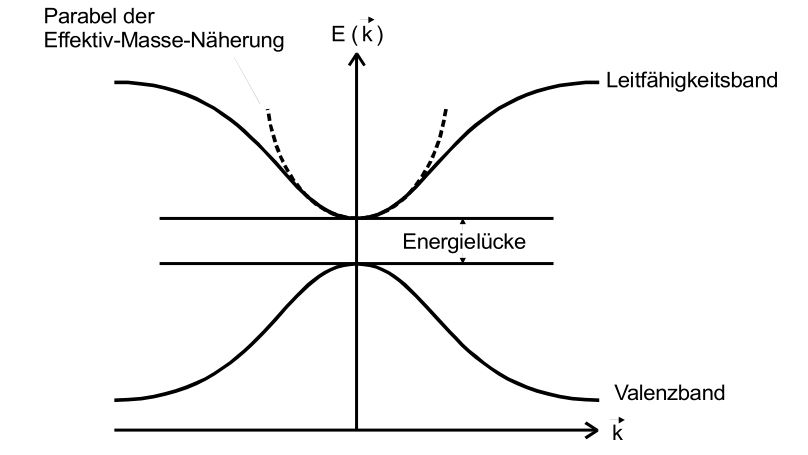
\includegraphics[width=0.4\textwidth]{Bilder/Energiebaender.jpg}
  \caption{Schematische Darstellung des Energiebandstruktur \cite{Anleitung}.}
  \label{T_Abb:1}
\end{figure}
Zur Beschreibung der Bandstruktur von Kristallen ist in es in vielen Fällen hinreichend,
sich auf die untere Bandkante der Energiebänder zu beschränken (siehe Abbildung \ref{T_Abb:1}).
Der Verlauf der Energiebänder (entspricht der Elektronenenergie) wird mit einer Funktion
$\varepsilon(\vec{k})$ durch den Wellenzahlvektror $\vec{k}$ beschrieben. Diese, bei
Betrachtung des Gesammtverlaufs des Energiebandes in den meisten Fällen äußerst
komplizierte Funktion kann in der Nähe der Bandkante nach den Komponenten von $\vec{k}$
Taylorentwickelt werden. Sinniger Weise wird die Bandkante dabei in den Nullpunkt
des Koordinatensystems gelegt, sodass um Null entwickelt werden kann. Es folgt eine Taylorreihe:
\begin{equation}
  \varepsilon(\vec{k}) = \varepsilon(0) + \frac{1}{2} \sum_{i=1}^3 \left(
  \pdv[2]{\varepsilon}{k_i} \right)_{k=0} k_i^2 + \mathcal{O}(k_i^3).
  \label{T_eq:1}
\end{equation}
Weiterhin gilt die Beziehung
\begin{equation*}
  \varepsilon = \frac{\hbar^2 k^2}{2 m}
\end{equation*}
und ein Vergleich mit der Taylorreihe zeigt, dass die Größen:
\begin{equation*}
  m_i^* \coloneq \hbar^2 \left\{ \left(\pdv[2]{\varepsilon}{k_i} \right)_{k=0} \right\}^{-1}
\end{equation*}
Massen beschreiben. Diese Größen werden effektive Massen genannt und ermöglichen es,
dass Kristallelektronen als freie Elektronen betrachtet werden, wenn ihre Ruhemassen
in der Schrödingergleichung mit eben diesen effektiven Massen ersetzt werden. Das
Potential kann dann in guter Näherung vernachlässigt werden und für mäßige externe
Felder gilt das 2. $\textsc{Newtonsche}$ Axiom.\\
Für perfekte Kristallsymmetrien vereinfacht sich die Taylorentwicklung \eqref{T_eq:1}
dergestalt, dass aus den offensichtlich elliptischen Energieflächen kugelsymmetrische
werden (in diesem Fall gilt $k_x = k_y = k_z$).
Für solche Flächen lässt sich der $\textsc{Faraday}$-Effekt beschreiben.

\subsection{Zirkulare Doppelbrechung bei optisch aktiver Materie}
\begin{figure}[H]
  \center
  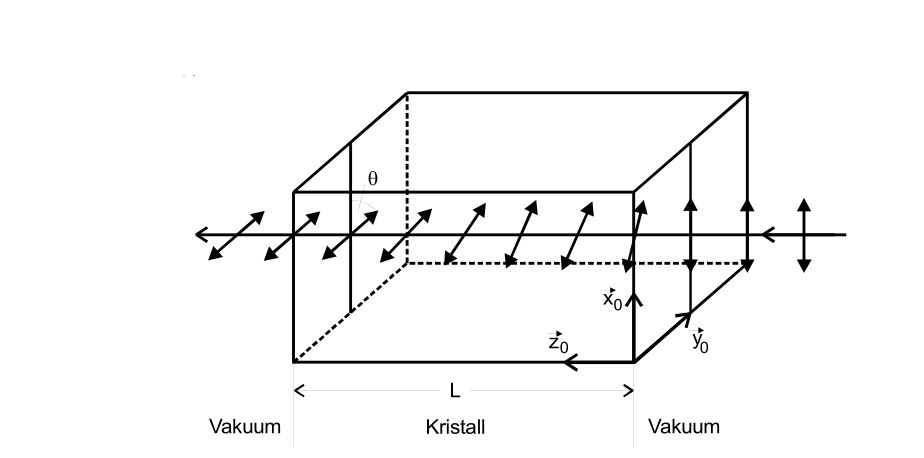
\includegraphics[width=0.4\textwidth]{Bilder/Kristall.jpg}
  \caption{Drehung der Polarisationsachse nach Durchgang durch ein optisch
  aktives Medium \cite{Anleitung}.}
  \label{T_Abb:2}
\end{figure}
Beim eintreten eines linear Polarisierten Lichtstrahls in ein optisch aktives Medium
wird die Polarisationsebene des Strahls gedreht. Dies lässt sich dadurch verstehen,
dass eine linear polarisierte Welle zu gleichen Teilen aus einem rechtszirkular und
einem linkszirkular zur Ausbreitungsrichtung (im folgenden $\vec{z}$) polarisierten
Teil besteht. Die beiden Zirkularisationsrichtungen breiten sich nun mit unterschiedlichen
Phasengeschwindigkeiten (bzw. Wellenzahlvektoren) aus und die linear polarisierte
Welle die nach durchgang durch den Kristall wieder austritt ist um den Winkel $\theta$
gedreht (siehe Abbildung [\textbf{??}]). Der Rotationswinkel berechnet sich zu
\begin{align*}
    \theta &=\frac{L}{2} \left(k_{\text{R}}-k_{\text{L}}\right)\\
          &=\frac{L\omega}{2}\left(\frac{1}{v_{\text{ph}_{\text{R}}}}-\frac{1}{v_{\text{ph}_{\text{L}}}}\right)\\
          &=\frac{L\omega}{2\text{c}}\left(n_{\text{R}}-n_{\text{L}}\right),
\end{align*}
wobei $v_{\text{ph}}=\omega k^{-1}$ die Phasengeschwindigkeit und $n=c v_{\text{ph}}^{-1}$
der Brechungsindex für links- bzw. rechtspolarisiertes Licht in einem Kristall der
Länge $L$ ist. Die Lichtfreuqenz der einlaufenden Welle ist durch $\omega$ gegeben.\\
Dieser, als zirkulare Doppelbrechung bezeichnete, Effekt geht auf im Kristallmedium induzierte
Dipole (permantente Dipole können der Frquenz des einfallenden Lichts nicht folgen) zurück.
Die Polarisation $\vec{P} = \varepsilon_0 \chi \vec{E}$ des Kristalls
steigt damit propotional zur dielektrischen Suszeptibilität
$\chi$. Für isotrope Materialien handelt es sich hier um eine skalare Größe, in anisotropen
Medien ist $\chi$ jedoch Richtungsabhängig und muss daher tensoriell definiert werden.
In vielen Fällen handelt es sich hier um eine Diagonalmatrix, das Material ist dann
nicht doppelbrechend (optisch inaktiv). Doppelbrechende Materialien weisen jedoch Nebenachseneinträge
auf, sodass $\chi$ in einfachen Fällen eine Gestallt:
\begin{equation*}
    \underline{\underline{\chi}} =
    \begin{pmatrix}
      \chi_{\text{xx}} & i\chi_{\text{xy}} & 0 \\
      -i \chi_{\text{xy}}& \chi_{\text{xx}} & 0 \\
      0& 0 & \chi_{\text{zz}}
      \end{pmatrix}
\end{equation*}
annimmt. Für den Drehwinkel nach Durchgang folgt dabei nach Taylorentwicklung in
erster Ordnung in guter Näherung:
\begin{equation}
  \theta = \frac{L \omega}{2 c n} \chi_{xy}.
  \label{T_eq:2}
\end{equation}

\subsection{Zirkulare Doppelbrechung bei optisch inaktiver Materie}
Als $\textsc{Faraday}$-Effekt wird nun das Auftreten des oben beschriebenen Effekts
bei optisch inakiver Materie bezeichnet, wenn ein äußeres Magnetfeld angelegt wird.
Aus der Bewegungsgleichung für ein gebundenes Elektron folgt bei Vernächlässigung
von Dämpfungseffekten und Feldeinflüssen durch das Lichtfeld für hohe
Lichtfrquenzen eine Verschiebungspolarisoation $\vec{P} = -N e_0 \vec{r}$.
Es lässt sich nun das in \eqref{T_eq:2} benötigte Tensorelement $\chi_{xy}$ bestimmen
und in guter Näherung folgt:
\begin{equation*}
  \theta(\lambda)=\frac{2\pi^2 \text{e}_0^3 \text{c}}{\epsilon_0}\frac{1}{m^2
  \lambda^2 \omega{_0}^4}\frac{N B L}{n}.
\end{equation*}
Hierbei wird durch $N$ die Anzahl der Elektronen pro Volumeneinheit, durch $B$
die externe Magentfeldstärke, durch $\lambda$ die Wellenlänge des einfallenden
Lichts und durch $\omega_0$ die meist im nahen infraroten liegende Resonanzfrequenz
der zu erzwungenen Schwingungen fähigen gebundenen Elektronen bezeichnet. Weiter
lässt sich im Limes $\omega_0 \rightarrow 0$ (also für freie Elektronen) ein Ausdruck
\begin{equation}
  \theta_{\text{frei}}(\lambda)=\frac{\text{e}_0^3}{8 \pi^2 \epsilon_0 \text{c}^3}
  \frac{\lambda^2}{m^2}\frac{N L B}{n}
  \label{T_eq:3}
\end{equation}
entwickeln. Dieser kann unter Verwendung der oben eingeführten effektiven Masse
auch für Kristallelektronen verwendet und zur Bestimmung ebendieser genutzt werden.

\section{Durchführung}
\subsection{Versuchsaufbau}
\begin{figure}[H]
  \center
  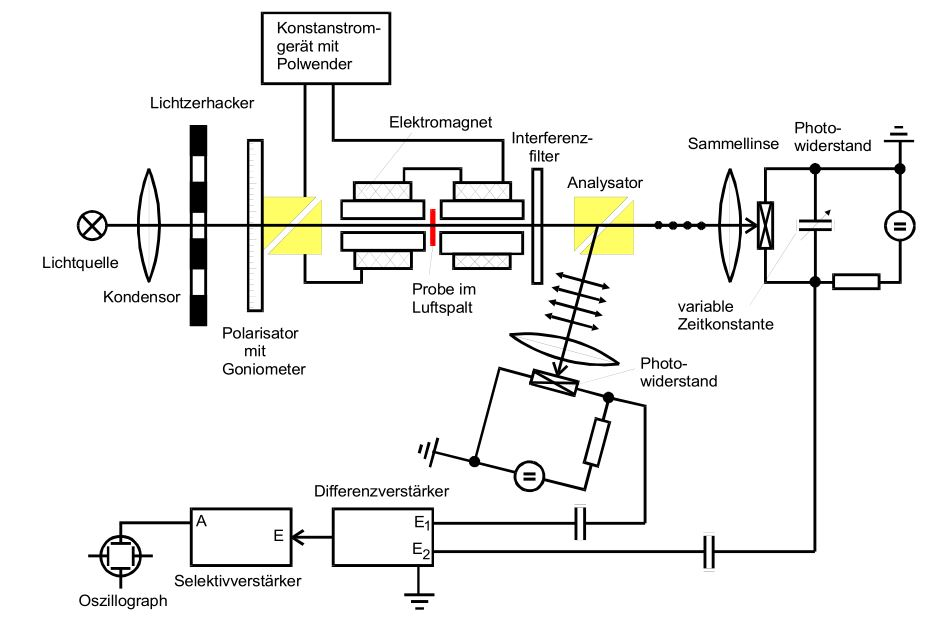
\includegraphics[width=0.8\textwidth]{Bilder/Aufbau.jpg}
  \caption{Schematische Darstellung des Versuchsaufbaus \cite{Anleitung}.}
  \label{D_Abb:1}
\end{figure}
Der Versuchsaufbau ist in Abbildung \ref{D_Abb:1} dargestellt. Das von einer Halogenlampe
emittierte Infrarotlicht wird über eine Kondensorlinse fokosiert,
durch einen Interferenzfilter monochromatisiert und durch
ein $\textsc{Glan-Thompson}$-Prisma (Polarisator) linear polarisiert. Die von diesem Licht durchleuchtete
Probe befindet sich dabei in einem Elektromagneten. Der Elektromagnet wird durch ein
Konstantspannungsgerät mit Strom versorgt. Integriert ist ein Polwender, der ein
gefahrloses Umpolen des Magnetfeldes ermöglicht, sodass die relative Magnetfeldänderung
auf $2B$ maximiert werden kann. Nach Durchlauf durch den Magneten trifft der Lichtstrahl
auf ein weiteres $\textsc{Glan-Thompson}$-Prisma (Analysator), durch welches der Strahl aufgespalten wird.
Beide Strahlen werden durch Sammellinsen auf Photowiderstände abgebildet. Damit an
den Photowiderständen eine Wechselspannung abfällt, wird ein Lichtzerhacker in den Strahlgang
eingebracht. Die abfallenden Spannungen werden auf einen Differenzverstärker
gegeben, der einem Selektivverstärker vorgelagert ist. Letzterer ist an die
Frequenz des Zerhackers gekoppelt. Der Ausgang des Selektivverstärkers wird letztlich
auf einem Oszilloskop dargestellt.

\subsection{Versuchsdurchführung}
Zu Anfang muss der Aufbau ohne Interferenzfilter und Probe justiert werden.
Nun wird in folgender Reihenfolge vorgegangen:
\begin{enumerate}
  \item Justage des Analysator-Prismas:\\
  Das Analysator-Prisma wird so um seine vertikale Achse gedreht, dass
  der gerade durch das Prisma gehende Strahl bei geeigneter Stellung des
  Polarisator-Prismas verschwindet.
  \item Justage der Photowiederstände:\\
  Die relative Position zwischen den Photowiederständen und den vorgelagerten
  Sammellinsen wird so einjustiert, dass die einfallenden Strahlen gut auf
  die Photowiderstände abgebildet werden.
  \item Jusatge von Selektivverstärker:\\
  Der Zerhacker wird eingeschaltet und die gewählte Frequenz am Selektivverstärker
  eingestellt. Der Differenzverstärker wird dafür durchgeschaltet. Das Ausgangssignal wird
  nun auf dem Oszilloskop beobachtet und  der Selektivverstärker zu eingeregelt,
  dass das Signal maximal wird. Sollte der Rauschanteil nicht ausreichend stark
  herausgefiltert werden, muss ein Lock-In-Verstärker eingeschleift werden.
  \item Helligkeitsjustage:\\
  Position von Lichtquelle und Linse werden so gewählt, dass die Lichtintensität
  besser wird.
  \item Überprüfen der Apperatur:\\
  Es werden Probe und Interferenzfilter eingesetzt und unter Variation von
  Polarisatorstellung und Zeitkonstante eines Photowiderstands geprüft,
  ob am Selektivverstärker ein Signal abfällt, dass, bis auf Störspannungen, null ist.
\end{enumerate}
Nach der Justage das maximale Magnetfeld in Strahlrichtung mit einer Hallsonde gemessen. Danach wird
der Drehwinkel an n-dotiertem und hochreinem Galliumarsenit für mehrere Wellenlängen
im nahen Infrarot gemessen.\\
Der Drehwinkel wird dabei bestimmt, indem die Polarisatorstellung und die Zeitkonstanten der
Photowiderstände abwechselnd so eingestellt werden, dass am Differenzverstärker eine Spannung
Null abfällt. Die Winkelstellung des Polarisators wird abgelesen und die Messung
bei umgepolten Magnetfeld widerholt. Der Drehwinkel ergbiebt sich dann zu:
\begin{equation}
  \theta = \frac{1}{2} \left(\theta_1 - \theta_2 \right).
\end{equation}
\section{Auswertung}
\subsection{Fehlerrechnung}
\section{Diskusion}
\newpage
\nocite{*}
\printbibliography
